\documentclass{article}
\usepackage{listings}
\usepackage{graphicx}
\usepackage{tabto}
\usepackage{amsmath}
\usepackage[backend=biber]{biblatex}
\usepackage{caption}
\usepackage{subcaption}
\usepackage[english]{babel}

\usepackage{fontspec}
\usepackage{minted}
\usepackage{fancyvrb}

% \setsansfont{Calibri}
% \setmonofont{Consolas}

% **************** IMPORTANT NOTE *******************
%
% compile this file with the following command:
% xelatex -shell-escape project.tex
%
% ***************************************************

\addbibresource{project.bib}
%\bibliographystyle{ieeetr}

\begin{document}
\renewcommand{\theFancyVerbLine}{
  \sffamily\textcolor[rgb]{0.5,0.5,0.5}{\scriptsize\arabic{FancyVerbLine}}}


\title{ASE 396 Project}
\author{Dylan Pederson}

\maketitle

\section{Overview}

\subsection{Dynamics}

The purpose of this project is to estimate the state of a flying object (plane or UAV) using some nonlinear dynamics and a nonlinear measurement model. The dynamics model being employed for this system is the following

\begin{equation}\label{eqn:state_vector}
	\mathbf{x} = [x, y, z, \dot{x}, \dot{y}, \dot{z}, \omega]^T
\end{equation}

\begin{equation}\label{eqn:dynamics_model}
	\dot{\mathbf{x}} = \begin{bmatrix}
	       \dot{x} \\
	       \dot{y}\\
	       \dot{z}\\
	       -\omega\dot{y}\\
	       \omega\dot{x}\\
	       0\\
	       0
	\end{bmatrix}
	+ \mathbf{D}
	\begin{bmatrix}
		v_{\ddot{x}} \\
		v_{\ddot{y}} \\
		v_{\ddot{z}} \\
		v_{\omega}
	\end{bmatrix}
\end{equation}

\begin{equation}\label{eqn:discrete_turning}
	\omega_k = \omega_{k-1} + v_{\omega}
\end{equation}

where the matrix $\mathbf{D}=[0_{3x4}; I_{4x4}]$. In this model we will assume that the process noise is distributed as $v \sim \mathcal{N}(0, \mathbf{Q})$. We start with a prior distribution $\mathbf{x} \sim \mathcal{N}(\hat{x}_0, P_0)$ where

\begin{equation}\label{eqn:prior_mean}
	\hat{x}_0 = [0 m, 0 m, 0 m, 0 m/s, 0 m/s, 0 m/s, 10^{-3} rad/s]^T
\end{equation}

\begin{equation}\label{eqn:prior_cov}
	P_0 = diag[100 m^2, 100 m^2, 100 m^2, 10 m^2/s^2, 10 m^2/s^2, 10 m^2/s^2, 0.1 rad^2/s^2]
\end{equation}

Note here that this model assumes no control input, and that the process noise is uncorrelated in time. For the algorithm we identify the state transition matrix $\Phi(t_k,t_{k-1})$.


\begin{equation}\label{eqn:stm}
	\Phi(t_k,t_{k-1}) = 
	\begin{bmatrix}
		1 & 0 & 0 & \sin{\omega \Delta t}/\omega & -(1-\cos{\omega \Delta t})/\omega & 0 & 0 \\
		0 & 1 & 0 & (1-\cos{\omega \Delta t})/\omega & \sin{\omega \Delta t}/\omega & 0 & 0 \\
		0 & 0 & 1 & 0 & 0 & \Delta t & 0 \\
		0 & 0 & 0 & \cos{\omega \Delta t} & -\sin{\omega \Delta t} & 0 & \frac{\partial x}{\partial \omega} \\
		0 & 0 & 0 & \sin{\omega \Delta t} & \cos{\omega \Delta t} & 0 & \frac{\partial y}{\partial \omega} \\
		0 & 0 & 0 & 0 & 0 & 1 & 0 \\
		0 & 0 & 0 & 0 & 0 & 0 & 1
	\end{bmatrix}
\end{equation}

where $\frac{\partial x}{\partial \omega} = -\dot{y}\Delta t \cos{\omega \Delta t} - \dot{x}\Delta t \sin{\omega \Delta t}$ and $\frac{\partial y}{\partial \omega} = \dot{x}\Delta t \cos{\omega \Delta t} - \dot{y}\Delta t \sin{\omega \Delta t}$. When $\omega \rightarrow 0$, computer implementations have a problem with these formulae. In that case one can simply take $\lim_{\omega \rightarrow 0}$ of all the terms in $\Phi(t_k,t_{k-1})$ to get a 'safe' matrix. Similarly, we have the process noise transition matrix $\Gamma(t_k,t_{k-1})$.

\begin{equation}\label{eqn:pntm}
	\Gamma(t_k,t_{k-1}) = 
	\begin{bmatrix}
		(1-\cos{\omega \Delta t})/\omega^2 & -(\omega\Delta t-\sin{\omega \Delta t})/\omega^2 & 0 & 0 \\
		(\omega\Delta t-\sin{\omega \Delta t})/\omega^2 & (1-\cos{\omega \Delta t})/\omega^2 & 0 & 0 \\
		0 & 0 & \Delta t^2/2 & 0 \\
		\sin{\omega \Delta t}/\omega & -(1-\cos{\omega \Delta t})/\omega & 0 & 0 \\
		(1-\cos{\omega \Delta t})/\omega & \sin{\omega \Delta t}/\omega & 0 & 0 \\
		0 & 0 & \Delta t & 0 \\
		0 & 0 & 0 & \Delta t
	\end{bmatrix}
\end{equation}

One can easily verify that these matrices collapse to $I_{7x7}$ and $0_{7x4}$, respectively, when $\Delta t \rightarrow 0$.

\subsection{Measurement}

The measurement model consists of range $\rho$, azimuth $\alpha$, and elevation $\beta$ measurements, plus some measurement error $\mathbf{\epsilon}$.

\begin{equation}\label{eqn:measurement_model}
	\mathbf{z} = h(\mathbf{x}) + \mathbf{\epsilon}
\end{equation}

where $h(\mathbf{x}) = [\rho, \alpha, \beta]^T$. These measurement variables are related to the state variables by

\begin{equation}\label{eqn:range}
	\rho = \sqrt{(x-x_s)^2 + (y-y_s)^2 + (z-z_s)^2}
\end{equation}
\begin{equation}\label{eqn:azimuth}
	\alpha = tan^{-1}(\frac{x-x_s}{y-y_s})
\end{equation}
\begin{equation}\label{eqn:range}
	\beta = sin^{-1}(\frac{z-z_s}{\rho})
\end{equation}

where $x_s = [1000, 1000, 20]^T$. The errors are assumed to be distributed as $\epsilon \sim \mathcal{N}(0, \mathbf{R})$ where $\mathbf{R} = diag[0.5^2 m^2, 0.1^2 deg^2, 0.2^2 deg^2]$. Because these equations are nonlinear, yet still in a relatively simple analytical form, the Extended Kalman Filter will be employed. As such, we will need the measurement Jacobian

\begin{equation}\label{eqn:measurement_jacobian}
	\mathbf{H} = 
	\begin{bmatrix}
		\frac{x_r}{\rho} & \frac{y_r}{\rho} & \frac{z_r}{\rho} & 0 & 0 & 0 & 0 \\
		\frac{y_r}{x_r^2 + y_r^2} & \frac{-x_r}{x_r^2 + y_r^2} & 0 & 0 & 0 & 0 & 0 \\
		\frac{-x_r z_r}{\rho^2 \sqrt{\rho^2 - z_r^2}} & \frac{-y_r z_r}{\rho^2 \sqrt{\rho^2 - z_r^2}} & (1-\frac{z_r^2}{\rho^2})\frac{1}{\sqrt{\rho^2 - z_r^2}} & 0 & 0 & 0 & 0 \\
	\end{bmatrix}
\end{equation}

where $x_r$ is short hand notation for $(x-x_s)$, and similarly for $y_r$ and $z_r$.

\subsection{Extended Kalman Filter}

The Extended Kalman Filter (EKF) is formulated to handle nonlinear dynamics or measurement in such a way that will update a nonlinear state rather than a perturbation to a linear dynamic state. It works in two stages. First is a time update due to dynamics, also called the prediction update. Second is an update that leverages information due to a new measurement, also called the measurement update. The EKF time update consists of the following functional representation

\begin{equation}\label{eqn:update_control}
	[\mathbf{u}_{k-1}, G_{k-1}] = control(\Delta t, \hat{\mathbf{x}}_{k-1})
\end{equation}
\begin{equation}\label{eqn:update_process_noise}
	[\bar{\mathbf{v}}_{k-1}, \mathbf{Q}_{k-1}, \Gamma(t_k,t_{k-1})] = process\_noise(\Delta t, \hat{\mathbf{x}}_{k-1})
\end{equation}
\begin{equation}\label{eqn:update_dynamics}
	[\bar{\mathbf{x}}_k^*, \Phi(t_k,t_{k-1})] = dynamics(\Delta t, \hat{\mathbf{x}}_{k-1}, \mathbf{u}_{k-1}, \bar{\mathbf{v}}_{k-1})
\end{equation}

where here the dynamics are considered linear because we are considering the turning rate $\omega$ to be a discrete process (i.e. constant over any given time interval). This massively simplifies the dynamics update to be equivalent to the following

\begin{equation}\label{eqn:update_dynamics_simple}
	\bar{\mathbf{x}}_k^* = \Phi(t_k,t_{k-1})\hat{\mathbf{x}}_{k-1} + \Gamma(t_k,t_{k-1})\bar{\mathbf{v}}_{k-1}
\end{equation}
\begin{equation}\label{eqn:update_covariance}
	\bar{\mathbf{P}}_k = \Phi(t_k,t_{k-1}) \mathbf{P}_{k-1} \Phi(t_k,t_{k-1})^T + \Gamma(t_k,t_{k-1}) \mathbf{Q}_{k-1} \Gamma(t_k,t_{k-1})^T
\end{equation}

Then the measurement model is used as follows
\begin{equation}\label{eqn:measurement}
	[h(\bar{\mathbf{x}}_k^*), \mathbf{H}_k, \Delta z] = measurement\_model(\bar{\mathbf{x}}_k^*, z_k)
\end{equation}
where $\Delta z = z_k - h(\bar{\mathbf{x}}_k^*)$ and $\mathbf{H}_k = \mathbf{H}(\bar{\mathbf{x}}_k^*)$. Finally, the measurement update is performed 

\begin{equation}\label{eqn:measurement_gain}
	%\bar{\mathbf{P}}_k = 
	\mathbf{K}_k = \bar{\mathbf{P}}_k \mathbf{H}_k^T(\mathbf{H}_k \bar{\mathbf{P}}_k \mathbf{H}_k^T + \mathbf{R})^{-1}
\end{equation}
\begin{equation}\label{eqn:measurement_state}
	\hat{\mathbf{x}}_k = \bar{\mathbf{x}}_k^* + \mathbf{K}_k \Delta z
\end{equation}
\begin{equation}\label{eqn:measurement_covariance}
	\mathbf{P}_k = \bar{\mathbf{P}}_k - \mathbf{K}_k \mathbf{H}_k \bar{\mathbf{P}}_k
\end{equation}

and the algorithm is repeated for new measurements. 
\section{Tuning}

The process noise covariance $\mathbf{Q}$ is a free variable that can be changed to 'tune' the filter. In this spirit, a sweep of values of $\mathbf{Q}$ is performed to choose the 'optimal' value. The suggested starting value for $\mathbf{Q}$ is 

\begin{equation}\label{eqn:Q_init}
	\mathbf{Q}_0 = diag[10^{-3} m^2/s^4, 10^{-3} m^2/s^4, 10^{-3} m^2/s^4, 10^{-7} rad^2/s^4]
\end{equation}

The tuning procedure consists of varying the value $a$ where

\begin{equation}\label{eqn:Q}
	\mathbf{Q} = a\mathbf{Q}_0
\end{equation}

Then after the filter has run with a given $\mathbf{Q}$, the mean and standard deviation of the post-fit residuals are analyzed to find the optimal value for $a$.

\begin{figure}[!htbp]
	\centering
	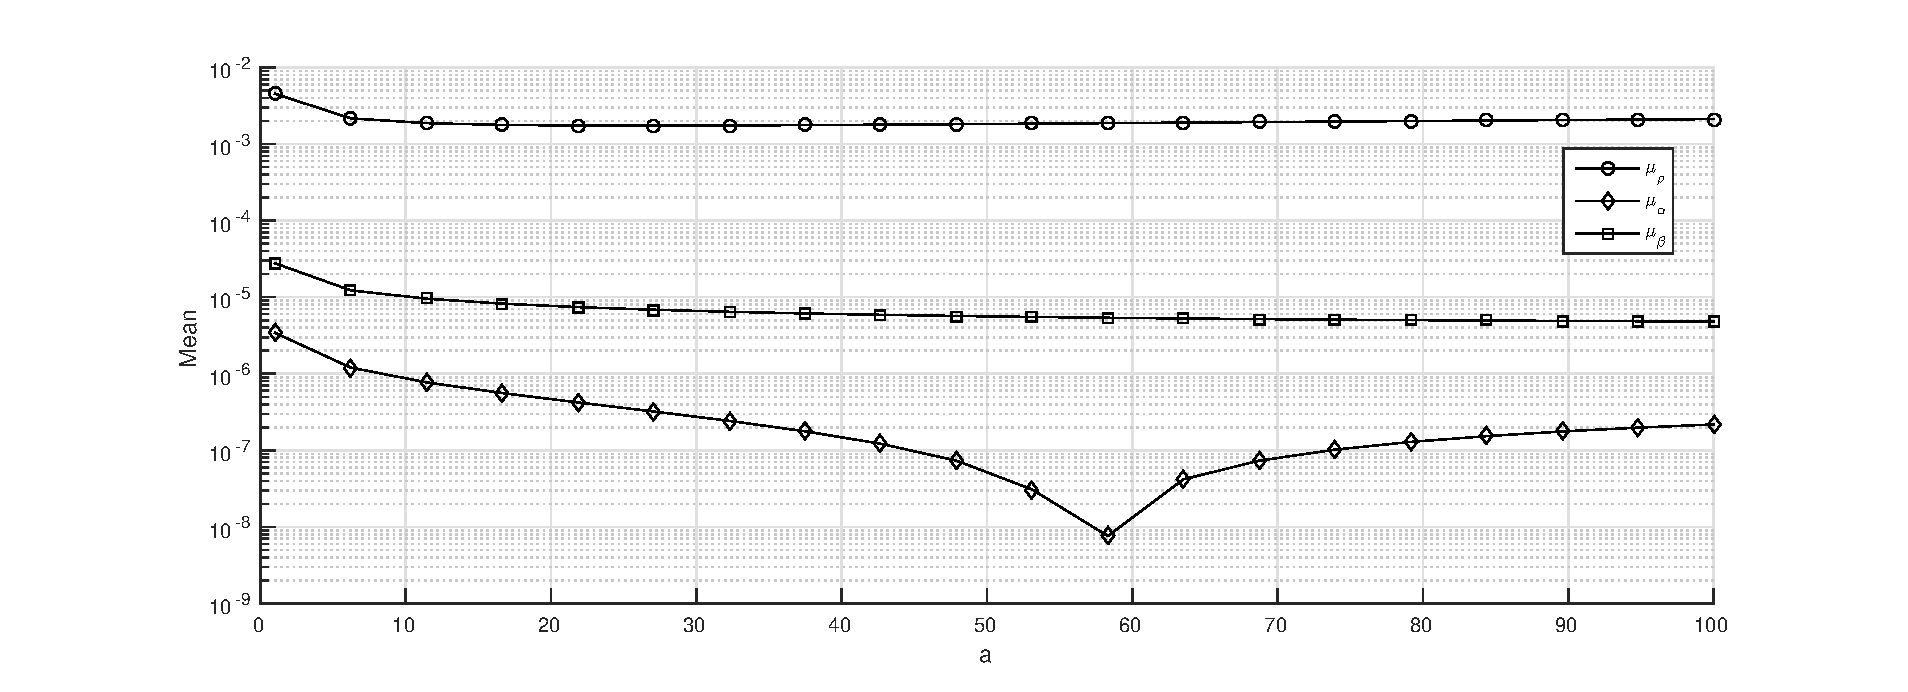
\includegraphics[scale=0.5]{figs/tuning_mean.eps}
	\caption{Mean of the post-fit residuals with varying $a$}
	\label{fig:tuning_mean}
\end{figure}

\begin{figure}[!htbp]
	\centering
	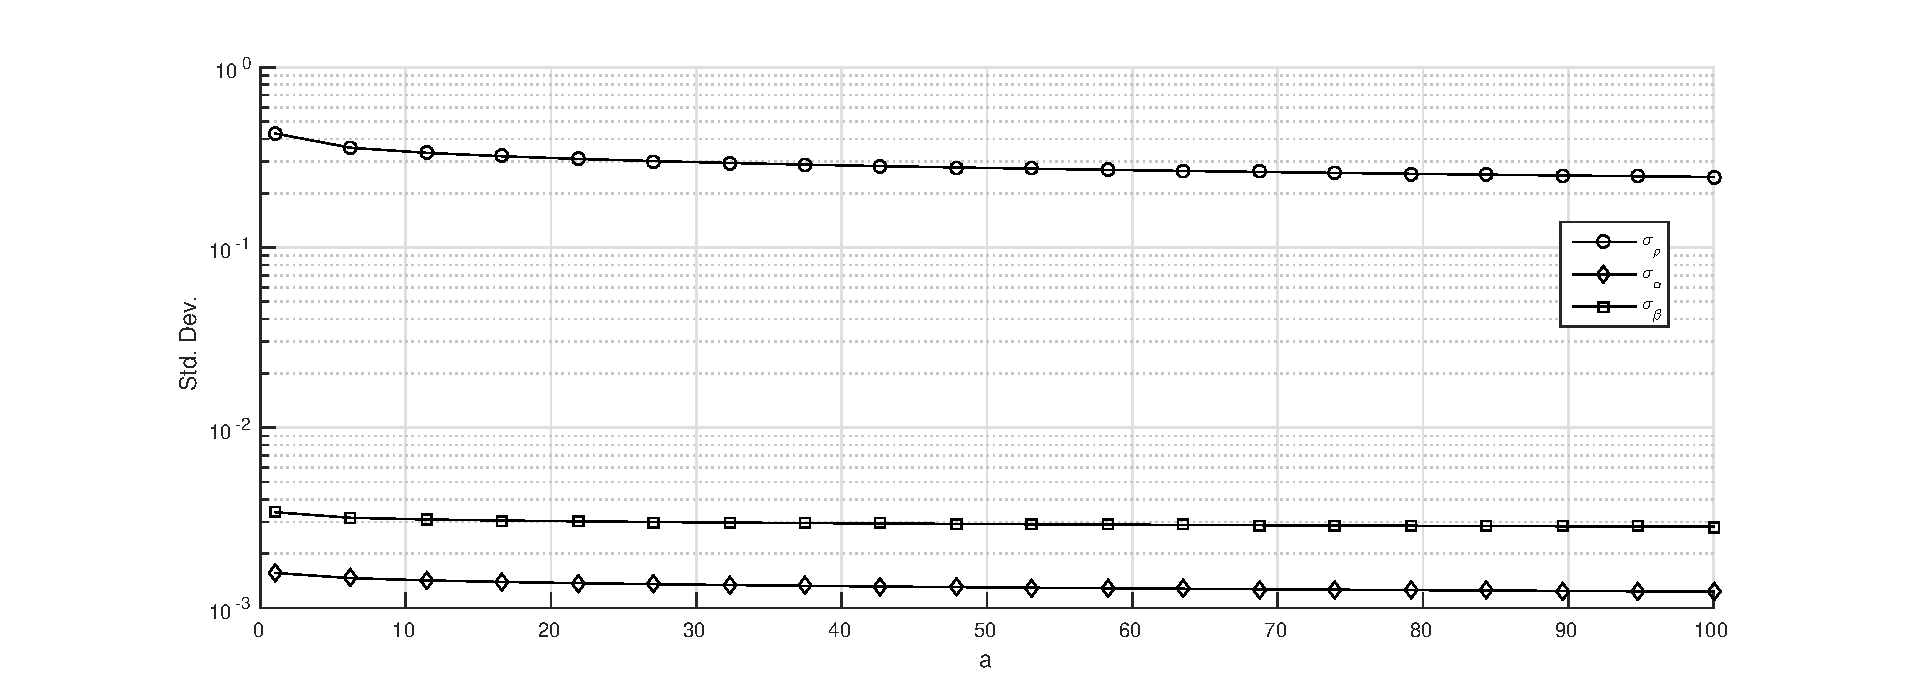
\includegraphics[scale=0.5]{figs/tuning_stddev.eps}
	\caption{Standard deviation of the post-fit residuals with varying $a$}
	\label{fig:tuning_stddev}
\end{figure}

From Figures ~\ref{fig:tuning_mean} and ~\ref{fig:tuning_stddev} we can identify a couple of optimal points. The mean of the post-fit residuals for $\rho$ is at its closest point to 0 around $a=20$, whereas the mean of the post-fit for $\alpha$ is at its closest point to 0 around $a=60$. The standard deviations of the post-fit residuals all keep decreasing with larger $a$. Given that the residual for $\rho$ is orders of magnitude larger than that for $\alpha$, we will use the point $a=20$ as the optimum.

% \begin{multline*} 
% \frac{{D}_x|_{i+1/2,j,k}^{n+1} - {D}_x|_{i+1/2,j,k}^{n}}{\Delta t} = [\frac{{H}_z|_{i+1/2,j+1/2,k}^{n+1/2} - {H}_z|_{i+1/2,j-1/2,k}^{n+1/2}}{\Delta y} \\
% - \frac{{H}_y|_{i+1/2,j,k+1/2}^{n+1/2} - {H}_y|_{i+1/2,j-1/2,k-1/2}^{n+1/2}}{\Delta z}] - c_0J_{e,x}|_{i+1/2,j,k}^{n+1/2}
% \end{multline*} 


% \begin{itemize}
% 	\item radiation boundary condition
% 	\item arbirtrarily complex material dispersion
% 	\item plane wave source condition
% 	\item arbitrary source frequency content
% \end{itemize}


\section{Discussion}

Using the selected value of $a=20$ for the process noise covariance $\mathbf{Q}$, we get the trajectory shown in Figure ~\ref{fig:trajectory}.

\begin{figure}[!htbp]
	\centering
	\includegraphics[scale=0.5]{figs/trajectory.eps}
	\caption{Trajectory after filter tuning}
	\label{fig:trajectory}
\end{figure}


This trajectory looks reasonably continuous and sensible from an intuitive standpoint. To gain more insight into the accuracy of the filter, we examine the residuals and the covariance.

\begin{figure}[!htbp]
	\centering
	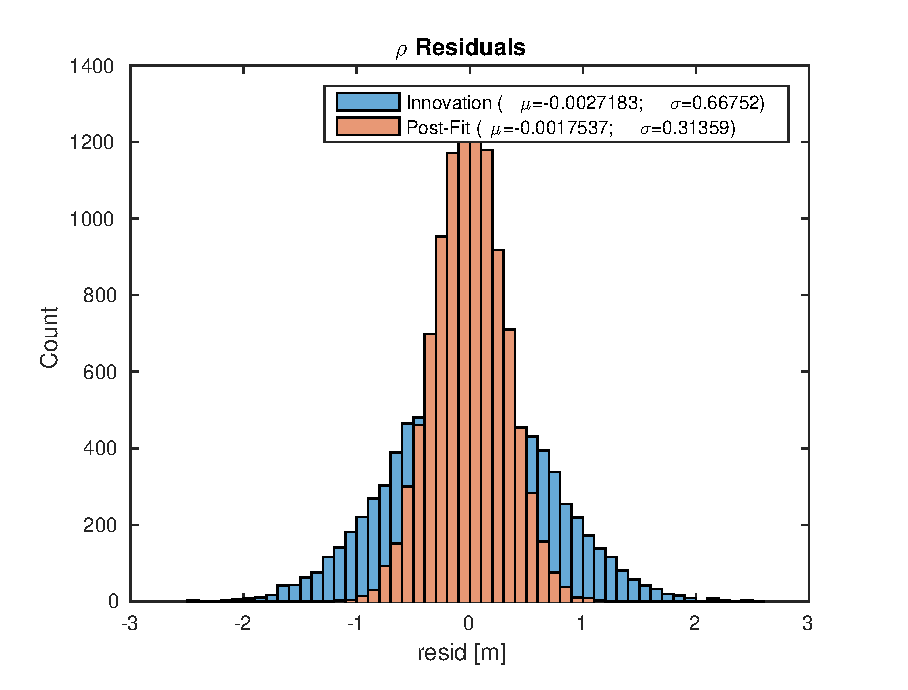
\includegraphics[scale=0.7]{figs/resid_rho.eps}
	\caption{residuals in the range}
	\label{fig:resid_rho}
\end{figure}

\begin{figure}[!htbp]
	\centering
	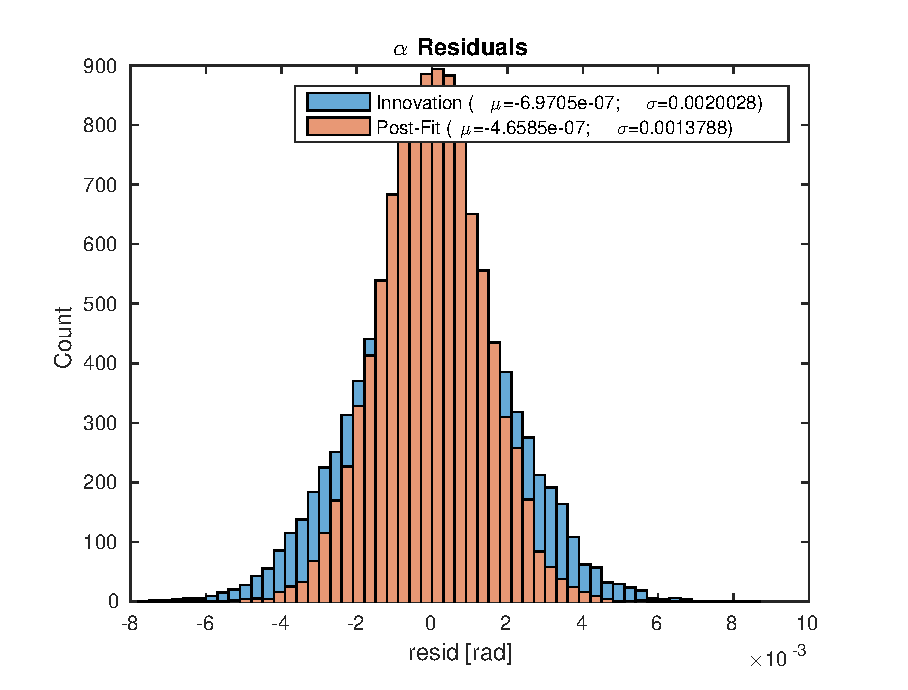
\includegraphics[scale=0.7]{figs/resid_alpha.eps}
	\caption{residuals in the azimuth}
	\label{fig:resid_alpha}
\end{figure}

\begin{figure}[!htbp]
	\centering
	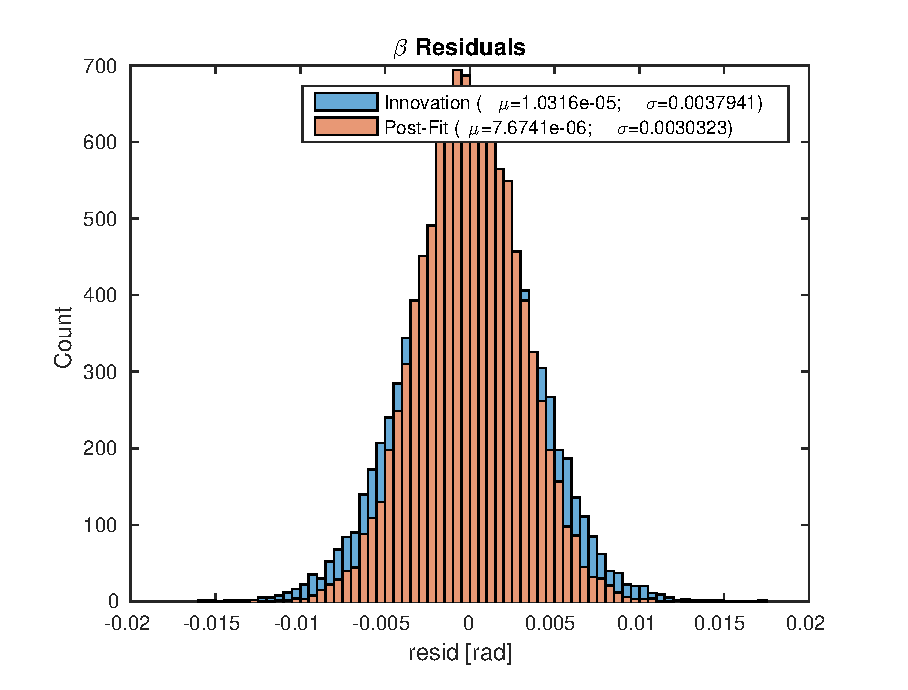
\includegraphics[scale=0.7]{figs/resid_beta.eps}
	\caption{residuals in the elevation}
	\label{fig:resid_beta}
\end{figure}

\begin{figure}[!htbp]
	\centering
	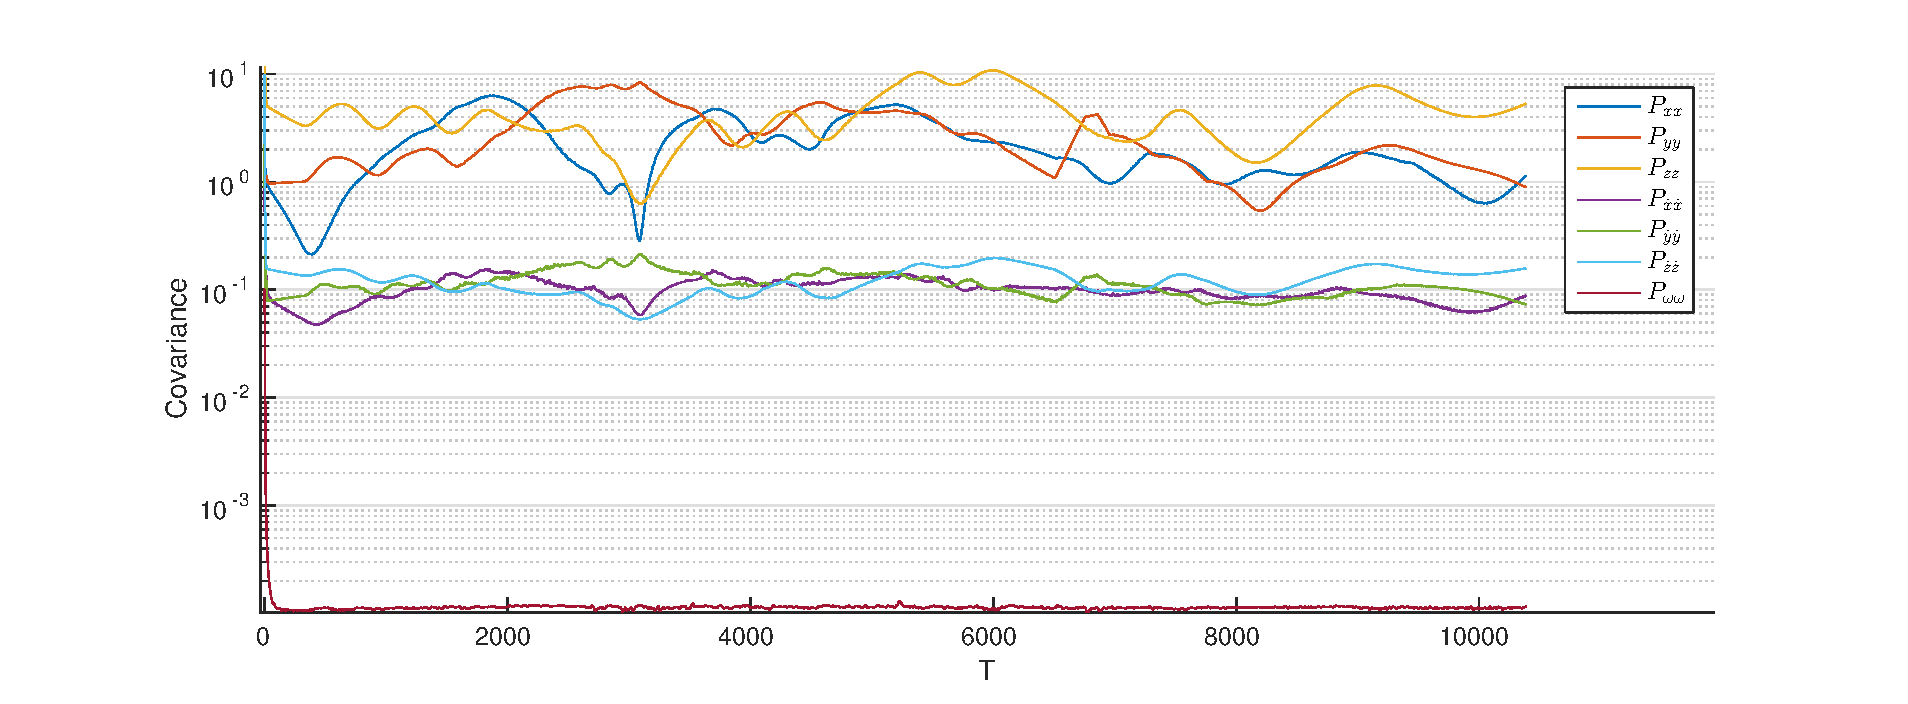
\includegraphics[scale=0.5]{figs/covariance.eps}
	\caption{Covariance values for each state variable over time}
	\label{fig:covariance}
\end{figure}

We observe that the residuals are approximately gaussian, centered at 0, and the post-fit residuals have a smaller variance than the innovations. We see that the post-fit residual has a much smaller variance than the innovation for the $\rho$ residuals, while the $\alpha$ and $\beta$ residuals have only slightly smaller variance. This reflects the fact that the observation errors in $\rho$ are small relative to its raw value. 

The covariance plots show that the covariance matrix $\mathbf{P}$ converges quickly, and stays stable throughout the total estimation time. There are some times (around $T=2000, 3000, 6000$) when the covariance becomes slightly larger for a brief moment. To understand this behavior, we look at the state and the raw measurements. 


\begin{figure}[!htbp]
	\centering
	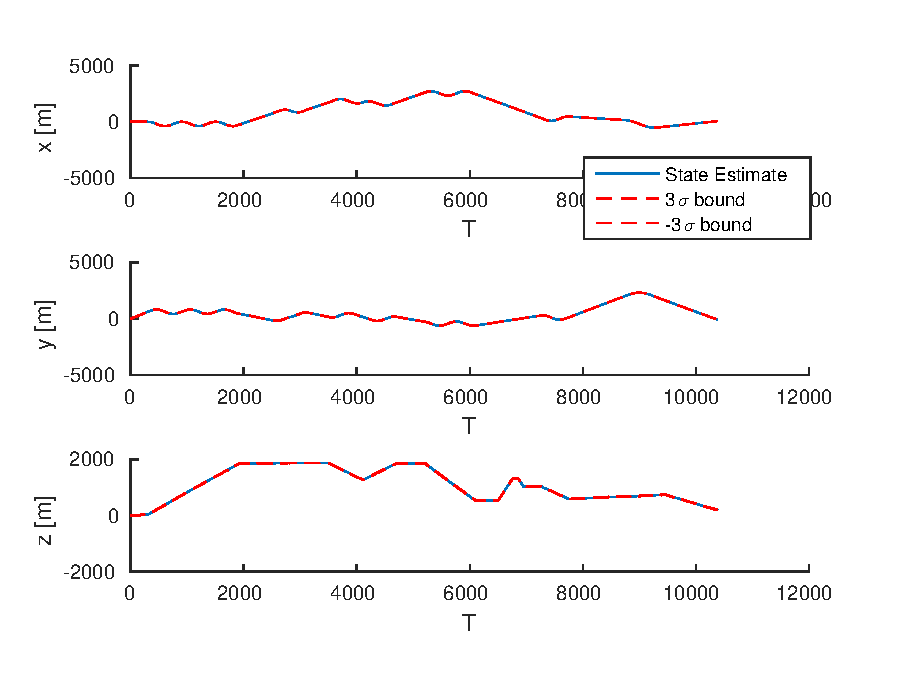
\includegraphics[scale=0.7]{figs/state_position.eps}
	\caption{State position over time}
	\label{fig:state_position}
\end{figure}

\begin{figure}[!htbp]
	\centering
	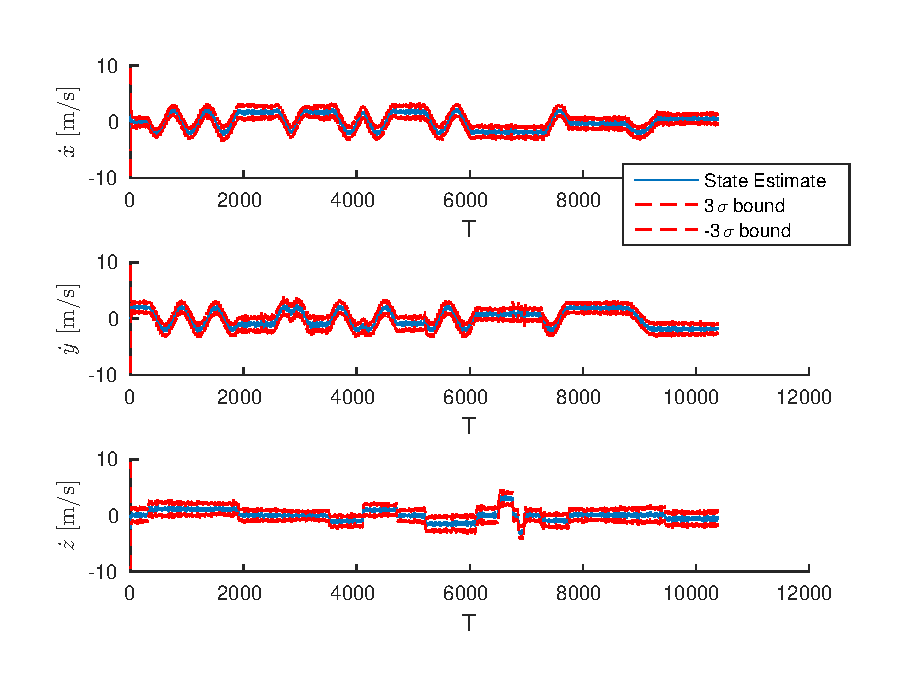
\includegraphics[scale=0.7]{figs/state_rate.eps}
	\caption{State rates over time}
	\label{fig:state_rate}
\end{figure}

\begin{figure}[!htbp]
	\centering
	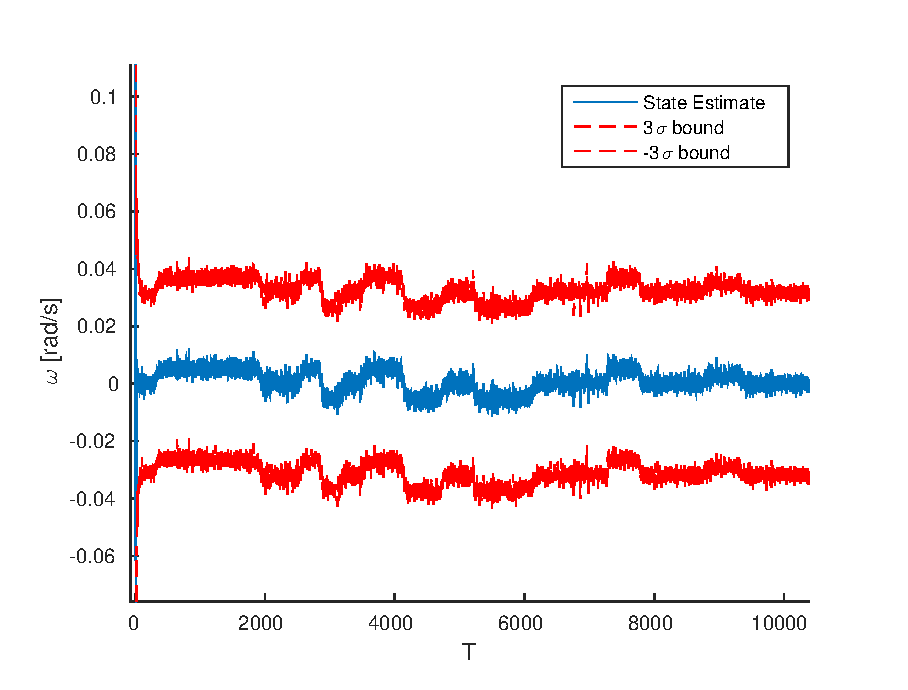
\includegraphics[scale=0.7]{figs/state_turning.eps}
	\caption{State turning rate $\omega$ over time}
	\label{fig:state_turning}
\end{figure}

\begin{figure}[!htbp]
	\centering
	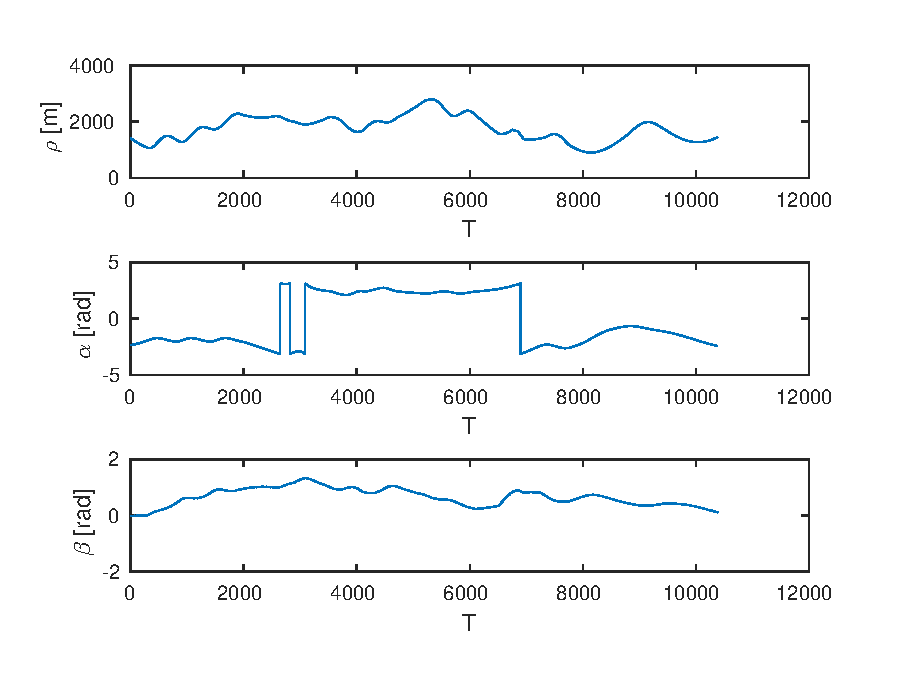
\includegraphics[scale=0.7]{figs/measurements.eps}
	\caption{measurement data over time}
	\label{fig:measurements}
\end{figure}

Looking at Figure ~\ref{fig:state_position} you can see that at approximately times $T=2000, 4000, 6000$ we have abrupt changes in $z$, whereas from Figure ~\ref{fig:state_turning}, we see an abrupt change in $\omega$ at time $T=3000$. It is possible that the increases in covariance at these times are due to abrupt control inputs that are not accounted for in the model (unknown). Because these control inputs cause a deviation from the predicted state, the covariance increases for a short while. 

% \lstinputlisting[language=C++, firstline=30, lastline=44]{exchange_sort.cpp}

% \section{Using MLE for \it{a priori}}



\section{Lessons Learned}

Through working on this project I learned that bounds checking on angular measurements is very important. Specifically, when calculating residuals, one must be careful to check bounds to be sure to get the correct difference. Another takeaway from this project was how to interpret a physical model with a discrete component ($\omega$). This was very confusing to me at first, because I wanted to do the usual way of taking the partials of the dynamics equation, then Laplace transforming. The method of solving for a 'reduced' set of equations of motion, then appending $\omega_k$ was new to me. It was also interesting to come up with a way to tune the filter. Surely there are many more sophisticated ways to do it (steepest descent optimization ?), but I lack the time to explore them. 




% \begin{figure}[h]
% \centering
% \includegraphics[scale=0.6]{figs/runtime.eps}
% \caption{Total runtime scaling behavior for the FDTD algorithm.}
% \end{figure}

% \begin{figure}[!h]
% \centering
% \includegraphics[scale=0.55]{figs/speedup.eps}
% \caption{Speedup for the FDTD algorithm.}
% \end{figure}

% \begin{figure}[!h]
% \centering
% \includegraphics[scale=0.6]{figs/efficiency.eps}
% \caption{Parallel Efficiency for the FDTD algorithm.}
% \end{figure}


\nocite{*}
\printbibliography


\section{Code}

\subsection{project.m}

\inputminted{matlab}{project.m}

\subsection{ExtendedKalmanFilter.m}

\inputminted{matlab}{ExtendedKalmanFilter.m}

\subsection{dynamics.m}

\inputminted{matlab}{dynamics.m}

\subsection{measurement.m}

\inputminted{matlab}{measurement.m}

\subsection{process\_noise.m}

\inputminted{matlab}{process_noise.m}

\subsection{zero\_control.m}

\inputminted{matlab}{zero_control.m}

\end{document}
